\documentclass[DIV12,english,11pt,halfparskip]{scrartcl}
\usepackage[pdftex]{graphicx}
\usepackage[latin1]{inputenc}
\usepackage[headsepline]{scrpage2}
\usepackage{amsmath}
\usepackage{amssymb}
\usepackage{graphicx}
\usepackage{xcolor}
\usepackage{natbib}
%\usepackage{subfigure}
\usepackage[pdfpagemode=None,%
%linkbordercolor = 0 0 0,%
linkcolor = red,%
%anchorcolor = 0 0 0,%
citecolor = blue,%
%filecolor = 0 0 0,%
%5menucolor = 0 0 0,%
%pagecolor = 0 0 0,%
urlcolor = violet,%
colorlinks,%
plainpages=false, pdfpagelabels,%
%backref,%
pdftitle={JANE - Annotation GUI},%
pdfsubject={},%
pdfauthor={Katrin Tomanek},%
pdfkeywords={Jena Annotation Environment, JANE},%
pdfcreator={JULIE Lab, University of Jena},%
pdfproducer={pdfeTeX},%
]{hyperref}
\pagestyle{scrheadings}
\automark{section}

\title{JANE -- Annotation GUI}

\author{\normalsize Katrin Tomanek ~~~~~~~~~~~~~ Alexander Klaue\\
  \normalsize  Jena University Language \& Information Engineering (JULIE) Lab\\
  \normalsize F\"urstengraben 30 \\
  \normalsize D-07743 Jena, Germany\\
  {\normalsize \tt \{tomanek|klaue\}@coling-uni-jena.de} } \date{}

\begin{document}
\maketitle
\newpage
\tableofcontents
\newpage

\section{Introduction}


This documentation is a user howto for the annotation GUI of JANE.
Throughout the documentation it is assumed that JANE annotation GUI is
installed on your PC. For installation, just unpack the GZIP-package,
change to folder \url{scripts} and run \url{configAnnoClient.sh} to
configure the annotation GUI settings. For details, please refer to
the installation howto. The annotation GUI has been tested on both
Windows (XP) and Linux (Ubuntu 7.*).


\subsection{Jena Annotation Environment}

The \emph{annotation GUI} (in the following also called
\emph{AnnoClient}) is part of the \emph{Jena Annotation Environment}
(JANE) which is a platform that supports the complete annotation
life-cycle and allows for `focused' annotation based on active
learning -- an intelligent selective sampling strategy that helps
reduce the amount of data to be annotated substantially at almost no
loss in annotation effectiveness.

JANE consists of several components, \textit{viz.} one central
component, the annotation repository, where all annotation and project
data is stored centrally, two user interfaces, namely one for the
annotators and one for the administrator, and the active learning
component (currently for named entity annotations only) which
interactively generates documents to speed up the annotation process.
All components communicate with the annotation repository through a
network socket -- allowing JANE to be run in a distributed
environment.


\subsection{Terminology}
\label{ss:terminology}
For a more detailed overview to JANE and its features, please refer to
\cite{Tomanek2007law}. In the following, we will shortly explain the
basic terminology used throughout this document.

An \textbf{annotation project} consists of a \textbf{collection of
  documents} to be annotated, an associated \textbf{annotation schema}
-- a specification of what has to be annotated in which way, according
to the accompanying annotation guidelines -- a set of configuration
parameters, and an \textbf{annotator} (or \textbf{user}) assigned to
it.

We distinguish two kinds of annotation projects: A \textbf{default
  project}, on the one hand, contains a predefined and fixed
collection of naturally occurring documents which the annotator
handles independently. In an \textbf{active learning
  (AL) project}, on the other hand, the annotator has access to
exactly one (AL-computed pseudo) document at a time. After such a
document has completely been annotated, a new one is dynamically
constructed which contains those sentences for annotation which are
the most informative ones for training a classifier.  Besides
annotators who actually do the annotation, there are
\textbf{administrators} who are in charge of (annotation) project
management (see administration GUI howto).




\subsection{Running the Annotation GUI}
In the subdirectory \url{scripts} of your \textsc{JANE} installation you
will find several command-line scripts. Run the annotation GUI by
executing the following script: \url{runAnnoClient.sh}.

\subsubsection{Login}
The annotation GUI now starts with a user login (see figure
\ref{fig:loginfigure}). All users which are currently added in the
annotation repository are shown here. After successfull login, the
main frame of the annotation GUI will open.

\begin{figure}[h]
  \centering
  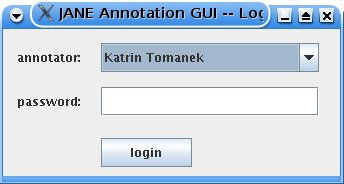
\includegraphics[scale=0.7]{figs/AnnoClientLogin.jpg}
  \caption{Annotation GUI login}
  \label{fig:loginfigure}
\end{figure}

\subsubsection{Logout}
Please not, that each user can only login once. This is a necessary
feature to avoid data inconsistency. Thus, you should close the GUI
properly and not just ``kill'' the GUI window. Only then the user is
logged out correctly. In case you did not logout properly (or the GUI
crashed for some reason), there is another command-line script which
can be used to logout a user: \url{logoutUser.sh}. Please, use this
script carefully always making sure that the user really should be
logged out!



\section{Annotation}
After successfull login, the main window opens (see figure
\ref{fig:annoclientfigure} ).

\begin{figure}[h]
  \centering
  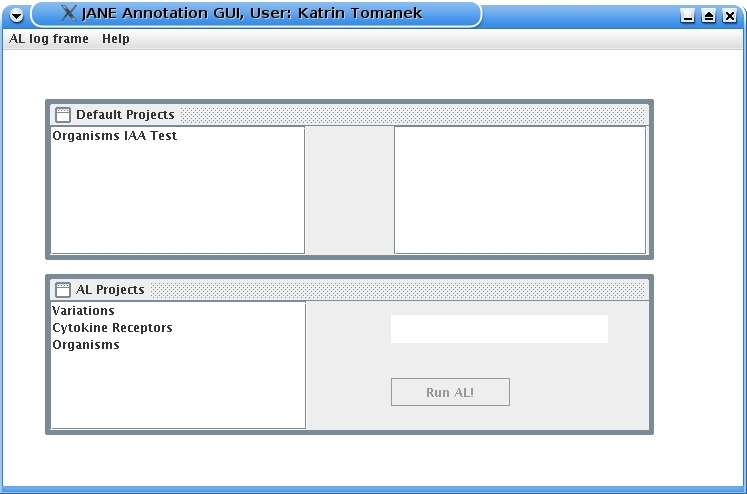
\includegraphics[scale=0.4]{figs/AnnoClientOnStartup.jpg}
  \caption{Main window of the annotation GUI}
  \label{fig:annoclientfigure}
\end{figure}

From the menu bar you can select the logging output of AL projects
(\textit{AL log frames}). The documentation can be viewed via the
\textit{Help} menu. Press the upper right button (mostly an ``X'',
depending on your window manager), to close the GUI and to
logout).

In the middle of the window, an overview over all projects assigned to
the current user is shown, ordered by the projects' respective mode
(default or AL project). See section \ref{ss:terminology} for a
description of these two types of projects.


\subsection{Default Projects}
With default projects, no active learning is possible. Double clicking
on such a project you will see all the documents that have been added
for annotation to this project (see figure \ref{fig:bdlist}).

\begin{figure}[h]
  \centering
  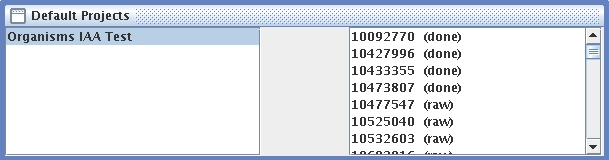
\includegraphics[scale=0.66]{figs/BaseDataList2.jpg}
  \caption{List of documents of selected default project.}
  \label{fig:bdlist}
\end{figure}


The documents can be flagged (\textit{done}, \textit{raw}, or
\textit{in progress}). A right-click on the respective document will
popup a small menu where you can change the status (see figure
\ref{fig:bdstatus}). After complete annotation of a document it
\emph{should} be set to \emph{done} as only documents with this flag
are considered by some operations from the administration GUI (as
e.g. deployment and inter-annotator agreement calculations).

\begin{figure}[h]
  \centering
  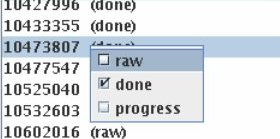
\includegraphics[scale=0.9]{figs/BaseDataStatus.jpg}
  \caption{Setting the annotation status of documents.}
  \label{fig:bdstatus}
\end{figure}


\subsection{AL Projects}
% - for NER especially, also other segmentation tasks possible

Focused selection of the text units to be annotated, known as active
learning selection, is limited to AL projects. Please note, that at the
moment, AL-selection is only supported for segmentation task
annotations and is actually tuned to entity mention annotations.

In contrast to default projects, an AL project has only one document
(which is a artificially compiled document consisting of sentences
that were selected from different documents) is available at one time.
Double-clicking in an AL project we are shown this document on the
right side (see figure \ref{fig:alproject}).

Further, in the right side of the AL project frame, there is an
additional button stating \textit{Run AL!}. Once the document is
completely annotated and its status has been set to
\emph{done}\footnote{Annotating an AL project and changing its status
  works exactly in the same way as with an default project.} this
button is enabled (otherwise it disabled and has a light-gray color)
allowing you to request a new document from the \emph{active learning
  component}.

\begin{figure}[h]
  \centering
  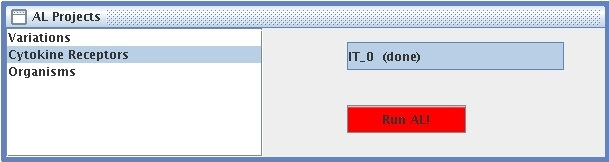
\includegraphics[scale=0.66]{figs/ALButton2.jpg}
  \caption{AL project with current document and AL button.}
  \label{fig:alproject}
\end{figure}

Once the annotator has pressed the AL button, active learning is started
for selected project. A new frame with AL logging information telling
the current status of the active learning selection is shown. This
frame can manually be closed and reopend via the menu bar (\textit{AL
  log frames}). 

When AL selection has been started the AL button turns into a number
telling the estimated time that AL selection will probably
take\footnote{However note, that the prediction of the AL selectiont
  time is only a very rough measure.} (see figure
\ref{fig:alselection}). AL selection can take a while, depending on
the number of documents that have already been annotated: 2-10 minutes
selection time are usual.

During the AL selection, the current AL project cannot be edited, but
is locked and gray-colored. However, the user can work on other
projects in the mean-time: he could for example annotate a default
project\footnote{Infact, active learning can be started and run for
  all other AL-projects at the same time, however, users should be
  warned that when more than one AL selection is started by the same
  user, the AL logging does not work properly as well the the
  estimation of the AL selection time.}.  Of course, the annotation
GUI can be closed and restarted while the AL selection is running.
This doesn't affect the AL selection.

When AL selection is finished, the current AL project is again
editable and the AL button is again labeled \emph{Run AL!} (instead of
with the estimated time). A new document (named e.g. \emph{IT-5}
for AL iteration 5) is than displayed for the respective project.

\begin{figure}[h]
  \centering
  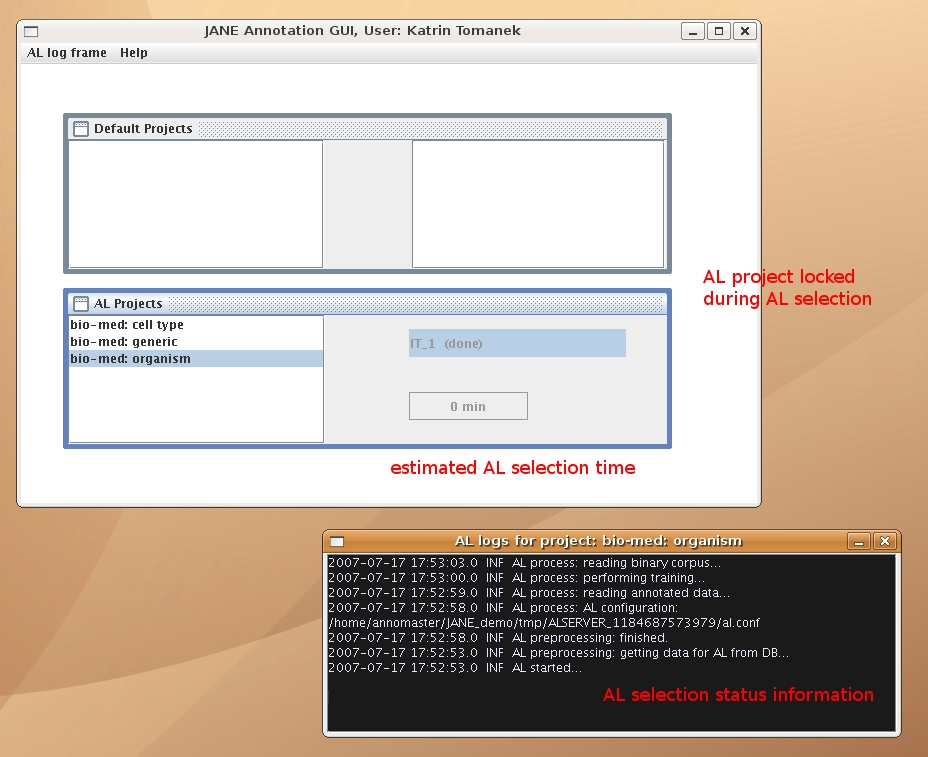
\includegraphics[scale=0.5]{figs/ALSelection.jpg}
  \caption{AL project locked while AL selection is running.}
  \label{fig:alselection}
\end{figure}



\subsection{Annotating in External Editor}
Till now, we have only described several operations, however not the
annotation itself. Annotation it done using the external annotation
editor MMAX2\footnote{MMAX2 was originally developed at the European
  Media Lab and is now an open source project, see
  \url{http://mmax2.sourceforge.net}}

In both default and AL projects, the annotation editor is started by
double-clicking on a selected document in the list. It might take some
seconds for MMAX2 to open, get rid of the validation window by just
clicking ``Do not validate.''. Now, the document you selected is now
shown in the editor's main window. 

While MMAX2 is running, the system autosaves the annotation in certain
time intervals. Note: Autosaving here means, that the current
annotations are uploaded to the annotation repository. In case MMAX2
(or the annotation GUI) crashes annotation can be continued at this
last ``checkpoint''. However, to make autosaving be effective the user
has to enable the autosaving option in MMAX2 or to manually save the
annotations in MMAX2 every now and then.

The user is informed via the \emph{MMAX2 output frame} whenever
autosaving is performed.  Further, any output MMAX2 (be it errors or
just information) is also shown in this frame. If, for example, MMAX2
has problems opening your document it will be shown there. 

While MMAX2 is running, the annotation GUI is inactive to avoid that
more than one annotation session is opened at a time by the same
user. Just close MMAX2 (and save your annotations) to return to the
annotation GUI. Remember to change the flags of the document you have
just annotated.

JANE stores the time needed to annotate a document. The annotation is
estimated from the time MMAX2 is opened for a document. This time is
shown also in the MMAX2 output frame after MMAX2 was closed.

Figure \ref{fig:mmax} shows an overview over the windows MMAX2
opens.\footnote{Please refer to the MMAX2 documentation for a more
  detailed explanation of how to annotate with MMAX2.} We will here
only shortly discuss how to use MMAX2 for annotation:

\begin{figure}[tb]
  \centering
  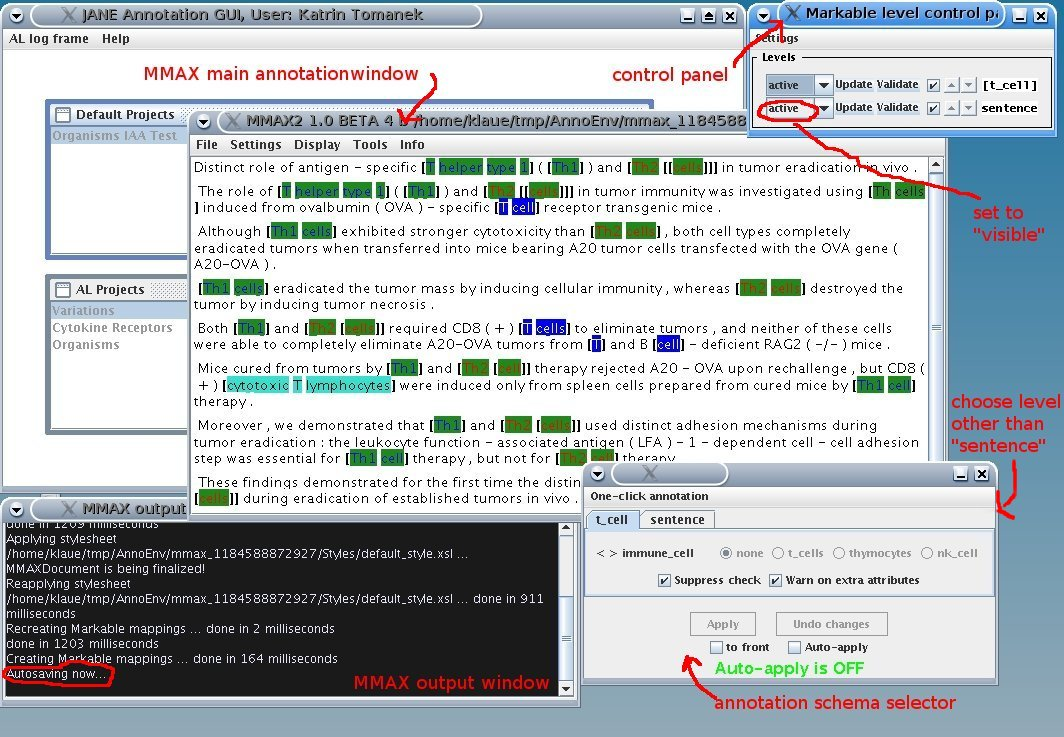
\includegraphics[scale=0.4]{figs/MMAX2.jpg}
  \caption{External annotation editor: MMAX2}
  \label{fig:mmax}
\end{figure}



After MMAX2 has started, go to the control panel window and change the
mode for the \emph{sentence} level to visible (as you don't want to
annotate the sentence level but the other level, in our example e.g.
``t cells''). Further, go to the annotation schema window and also
select your according annotation schema here (if not selected already)
which will reveal the labels you can assign. Now you can make
annotations in your MMAX2 main annotation window: after having selected
some tokens from the text, you have to add a socalled \emph{Markable}
(an annotation in MMAX2 speak) for which you select from the annotation
schema window the appropriate label (don't forget to press the
\emph{Apply} button). Your annotations are now shown in colors.

\subsubsection{Important note: Annotation AL Projects} 

As MMAX2 allows chained annotations (important especially for any kind
of relation/event or e.g. coreference annotations, you can combine
several annotations. In an AL project you should \textbf{never}
combine annotations from different sentences. In such a case, AL
selection will crash. You will see an error in the AL logging window
stating that you did a \emph{``sentence overlapping
  annotations''}. The AL project is now internally set to error (the
AL button is disabled even though the project is set to \emph{done}).

When this happens, reopen MMAX2 for the critical document and revise
your annotations by removing that annotation (markable) that spanned
over more than one sentence.  Only after the removal of such
annotations AL selection can be run again.

Combining annotations from different sentences might happen
accidentally to unexperienced MMAX2 users: To avoid this, make sure
that when you want to make a new annotation, no other markable (i.e.
annotation) is currently selected. Please also refer to the MMAX2
manual.



\textbf{In AL projects}, the MMAX2 main annotation window contains many
sentences in italics. These sentences cannot be annotated but are
shown as the original context of the selected sentences.


\section{Copyright and License}

This software is Copyright (C) 2007 Jena University Language \&
Information Engineering Lab (Friedrich-Schiller University Jena,
Germany). It can be used free of charge for academic non-commercial,
non-profit research purposes only. If you want to use JANE other than
in the demo version you have to fill out and send us the license
agreement
(\url{https://watchtower.coling.uni-jena.de/~tomanek/coling/JANE/JULIE_JANE_LICENSE.pdf}).

JANE is provided on an ``as is'' basis, without any warranties or
conditions of any kind. Each recipient is solely responsible for
determining the appropriateness of using JANE.

Further, please note that JANE-1.2 is still a beta version!



\bibliographystyle{alpha}
\bibliography{literature}

\end{document}
